

\section{Experiments}
\label{others}
In this section, we first explore the meaning of the quality score learned by QAN. Then QAN's sensitivity to level of feature is analysed. Based on above knowledge, we evaluate QAN on two human re-identification benchmarks and two unconstrained face verification benchmarks. Finally, we analyse the concept learned by QAN and compare it with score labelled by human.
%\begin{figure}[h]
%  \label{fig-ped}
%  \centering
%  \includegraphics[width=12cm]{c5_experiment/dataset.pdf}
%  \caption{Samples of PRID2011 dataset and iLIDS-VID %dataset. Images in first row and second row belongs to %same person. So as images in third and fourth row.}
%\end{figure}



\subsection{What is learned in QAN?}


% Todo: fix this figure with typical samples
\textbf{Qualitative analysis} 
We visualize images with their $\mu$ generated by QAN to explore the meaning of $\mu$. Instances of same person with different qualities are shown in the first two rows in Fig.~\ref{fig:samples}. All images are selected from test set. The two images in the same column belong to a same person. The upper images are random selected from images with quality scores higher than 0.8 and the lower images are selected from images with quality scores lower than the corresponding higher one. It is easy to find that images with deformity, superposition, blur or extreme light condition tend to obtain lower quality scores than normal images.

The last two rows in Fig.~\ref{fig:samples} give some examples of other images random selected from test set. They are sorted by their quality scores from left to right. We can observe that instances with quality scores larger than 0.70 are easy to recognize by human while the others are hard. Especially many of hard images include two or more bodies in the center and we can hardly discriminate which one is the right target. 

\textbf{Quantitative analysis} 
In order to measure the relationship between the quality labelled by human and $\mu$ predicted by QAN, 1000 images in YouTube Face are selected randomly and the quality of them are rated subjectively by 6 volunteers, where each volunteer estimates a quality score for each image, ranging from 0 to 1. All the ratings of each volunteer are aligned by logistic regression. Then the 6 aligned scores of each image are averaged and finally normalized to $[0,1]$ to get the final quality score from human. %For each identity, Fig.~\ref{fig:ratings} shows five identities' faces in the whole set. We can see the score distributions of human and QAN are correlated. Faces with occlusion, blur, miss-align, abnormal pose and expression have lower scores both in human's score and QANs' score.


\begin{figure}[!htb]
\minipage{0.5\textwidth}
\centering
  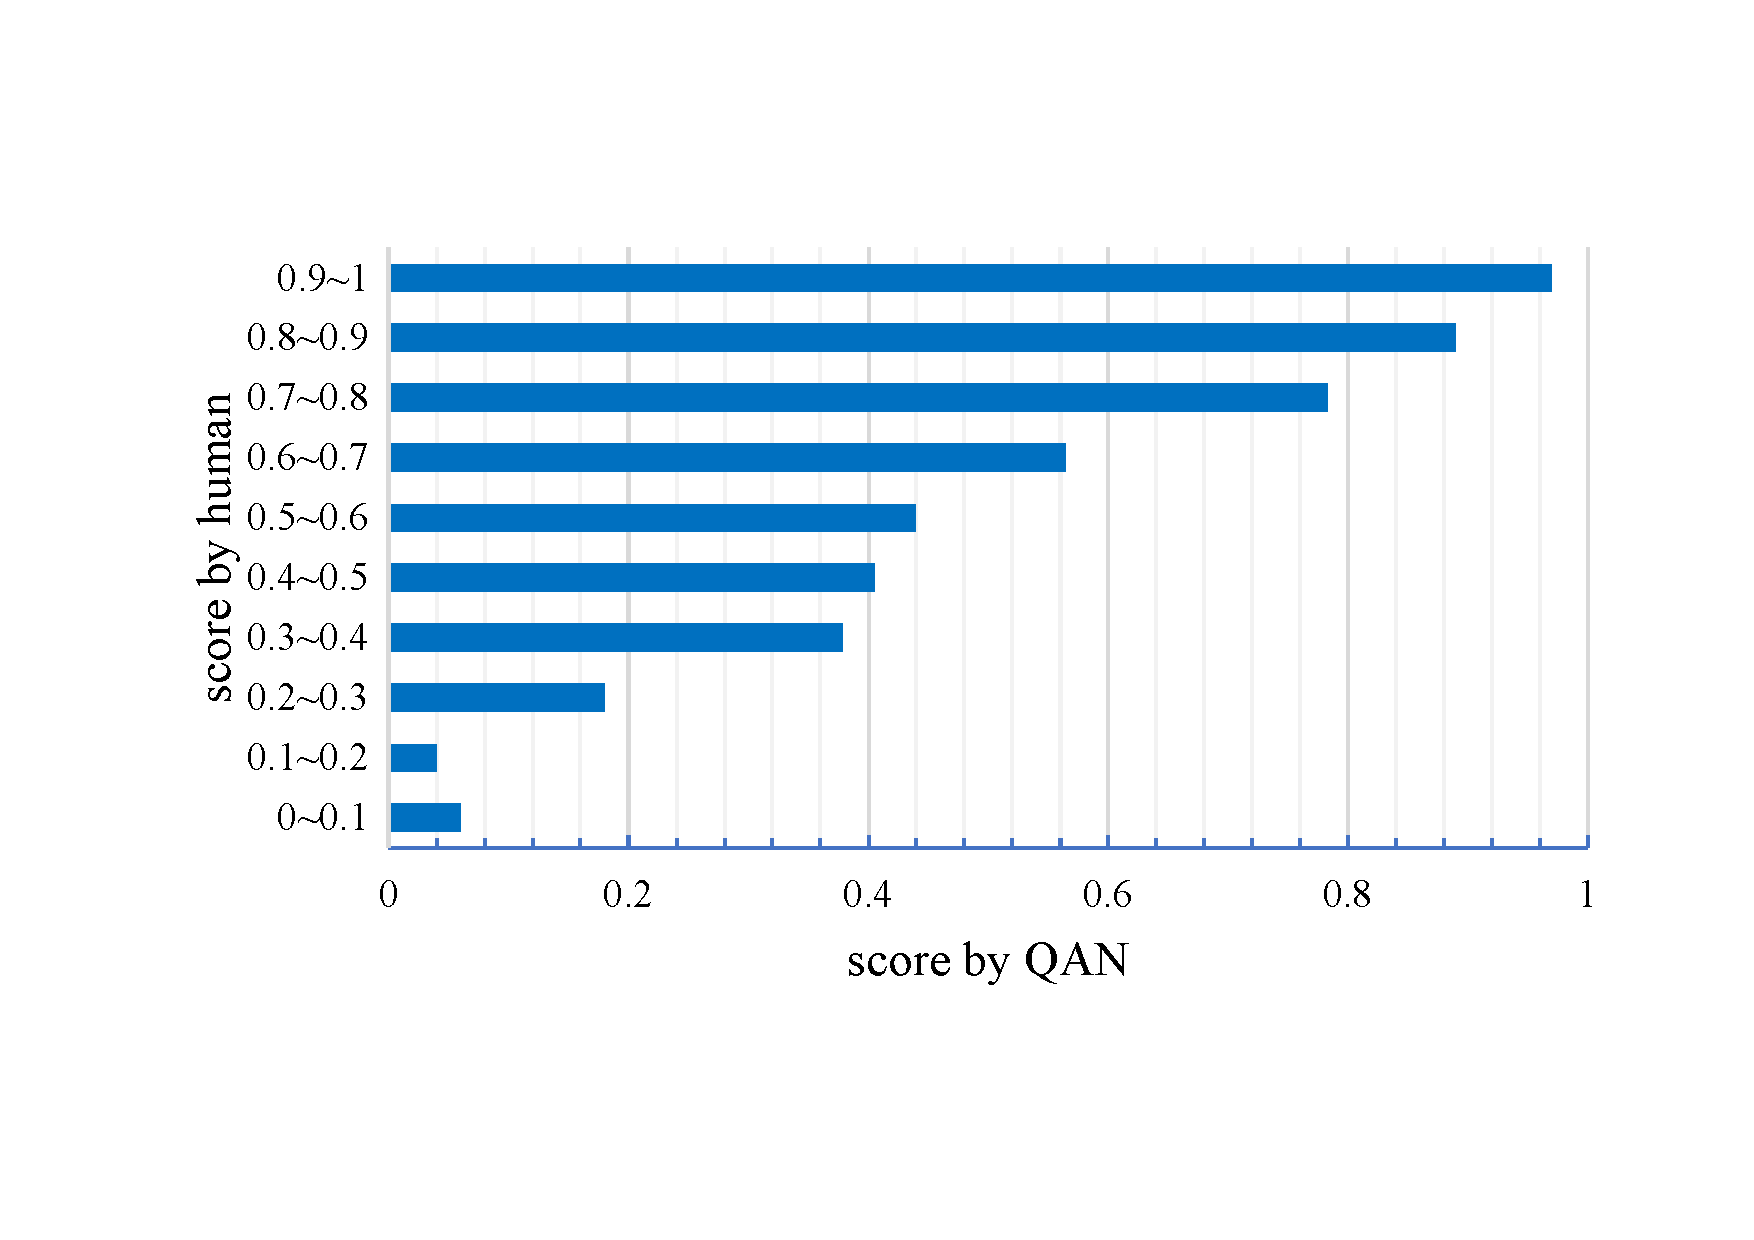
\includegraphics[width=9cm]{quality2.pdf}
  \caption{Comparison of qualities estimated by human and predicted by QAN.}
  \label{fig:quality}
\endminipage\hfill

%\minipage{0.32\textwidth}
%  \includegraphics[width=5cm]{c5_experiment/distribute1.pdf}
%  \caption{Distance distribution of features drawn from the output of QAN.}
%  \label{fig:subfig:a}
%\endminipage\hfill
%\minipage{0.32\textwidth}%
%  \includegraphics[width=5cm]{c5_experiment/distribute2.pdf}
%   \caption{Distance distribution of features directly drawn from feature generation module.}
%  \label{fig:subfig:b}
%\endminipage
\end{figure}

We divide the images into ten partitions based on human's score as shown in Fig.~\ref{fig:quality}. In which we show the corresponding quality statistics generated by QAN. It is obvious that the scores given by the QAN are strongly correlated with human-defined quality. We further analyse the 499,500 image pairs from these 1000 images and ask human and QAN to select the better one in each pair.  Result shows that the decision made by QAN has 78.1\% in common with human decision.

%From the analysis above, we can conclude that not only does the predicted quality score of QAN can represent the actual quality of an image, but also the criteria of human and QAN on the quality of image is mostly the same.

%\subsubsection{Cascade score generating unit influences feature extractor}

%\begin{figure}[ht]
%  \centering
%  \includegraphics[width=6cm]{c5_experiment/n4321-ok.pdf}
%  \caption{ROC curve comparison of QAN on YouTube Face dataset, using different score sources. QAN with human score performs better than the two baseline but worse than that scored by network.\label{fig:roc4321}}
%\end{figure}


%
%As discussed in Section~\ref{end2endtrain}, $Q(I)$ changes the distribution $G(I)$ fits. To explore how $Q(I)$ affects $G(I)$, we directly set the output of $Q(I)$ to be $1/N$, where $N$ is the number of images in a set. In this way, the output of this modified QAN is the average pooling of all images' features generated by $G(I)$, so we call this modified QAN as QAN-AvePool below. Then we use this QAN-AvePool's output as the representation of a image set and test its accuracy on YouTube dataset. As shown in Table~\ref{com_gi}, compared with original QAN and baseline, the feature extracted by QAN-AvePool has lower discrimination even than baseline model. At the false positive rate of $10^{-4}$, $10^{-3}$, $10^{-2}$ and $10^{-1}$, the true positive rate is 7.4\%, 3.2\%, 1.8\% and 0.7\% lower than the QAN.
%
%\begin{table}[h]
%\setlength{\abovecaptionskip}{10pt}
%\setlength{\belowcaptionskip}{10pt}
%  \label{com_gi}
%  \centering
%  \begin{tabular}{|l|c|c|c|}
%    \hline
%       TPR@FPR & 1e-3 & 1e-2  & 1e-1 \\
%    \hline
%       QAN-cascade2 	& \bf{0.7619} & \bf{0.8577} & \bf{0.9560} \\
%       CNN+AvePool 		& 0.6287 & 0.8279 & 0.9426 \\
%       QAN-AvePool 		& 0.5968 & 0.8094 & 0.9357 \\
%    \hline
%  \end{tabular}
%  \caption{Comparison of QAN, baseline and QAN-AvePool on YouTube Face dataset.}
%%\end{scriptsize}
%\end{table}
%
%
%To get an in-depth understanding of this performance drop, we draw the distance distribution of positive pairs (blue) and negative pairs (blue) in Fig.\ref{fig:subfig:a} and \ref{fig:subfig:b}. Result shows that the feature drawn directly from the feature generation part has larger variance on negative pair distance. This is within our expectation. Since hard samples get low scores from the score generation unit, according to Eq.~ \ref{11a},  the impact that hard samples make on gradient of $G(I)$ will be low in the back propagation process, so it is reasonable that $G(I)$ has lower discrimination than baseline. However, this influence is beneficial for set matching task for the prior that in each image set, there should be `good images' and `poor images', and QAN mainly focus on recognising ``good images'' and ignore the others, so it can improve the overall performance.









\subsection{Person re-identification}
\textbf{Datasets.} For person re-identification, we collect 134,942 frames with 16,133 people and 212,726 bounding boxes as the training data. Experiments are conducted on PRID2011~\cite{hirzer11a} and iLiDS-VID\cite{wang2014person} datasets. PRID2011 contains frames in two views captured at different positions of a street. \texttt{CameraA} has 385 identities while \texttt{CameraB} has 749 identities, and the two videos have a overlap of 200 people. Each person has 5 to 675 images, and the average number is 100. iLIDS-VID dataset has 300 people, and each person has two sets also captured from different positions. Each person has 23 to 192 images.

\textbf{Evaluation procedure.}
The results are reported in terms of \emph{Cumulative Matching Characteristics} (CMC) table, each column in which represents matching rate in a certain top-N matching.
Two settings are used for comprehensive evaluation. In the first setting, we follow the state-of-the-art method described in \cite{you2016top} and \cite{wang2016person}. The sets whose frame number is larger than 21 are used in PRID2011, and all the sets in iLIDS-VID are used. Each dataset is divided into two parts for fine-tuning and testing, respectively. For the testing set, sets form \texttt{CameraA} are taken as probe set while sets from \texttt{CameraB} are taken as the gallery. The final number is reported as the average of ``10-fold cross validation''. In the second setting, we conduct cross-dataset  testing. Different from the first setting, we ignore the finetuning process and use all data to test our model. That is, in PRID2011, the first 200 people from \texttt{CameraA} serve as probes, and all sets from \texttt{CameraB} are used as the gallery set. In iLIDS-VID,  \texttt{CameraA} are used as the probe set, and Camera B serve as gallery set.

\textbf{Baseline.}
We implement two baseline approaches. In the first baseline, we use average pooling to aggregate all images' representations. In the second baseline, a minimal cosine distance between two closures is used to be their similarity.

\subsubsection{Evaluation on common setting}

Results of evaluation obeying ``10-fold cross validation'' on  PRID2011 and iLIDS-VID are shown in Table~\ref{tab1} and Table~\ref{tab2}. Benefiting from the large scale training dataset, our CNN+AvePool and CNN+Min(cos) baselines are close to or even better than the state-of-the-art. Notice that most of the leading methods listed in table consider both appearance and spatio-temporal information while our method only considers appearance information. On PRID2011 dataset, QAN increase  top-1 matching rate by 11.1\% and 29.4\% compared with CNN+AvePool and CNN+Min(cos). On iLIDS-VID dataset, inherent noise is much more than that in PRID2011, which significantly influence the accuracy of CNN+Min(cos) since operator ``Min(cos)'' is more sensitive than ``AvePool'' to noisy samples . However, QAN achieves more gain on this noisy dataset. It increase top-1 matching rate by 12.21\% and 37.9\%. 

\begin{table}[!htb]
\normalsize
%\begin{scriptsize}
  \centering
  \begin{tabular}{l|c|c|c|c}
\hline
      \multicolumn{5}{c}{PRID2011}\\
    %\cmidrule{1-2}
\hline
       Methods & CMC1 &CMC5&CMC10 & CMC20 \\
\hline
       QAN 	& \textbf{90.3} & \textbf{98.2} & \textbf{99.32} & \textbf{100.0}  \\
       CNN+AvePool 		& 81.3 & 96.6 & 98.5 & 99.6 \\
       CNN+Min(cos) 		& 69.8 & 91.3 & 97.1 & 99.8  \\
\hline
       CNN+RNN\cite{wu2016deep} & 70 & 90 & 95 & 97  \\
       STFV3D\cite{liu2015spatio} & 42.1 & 71.9 & 84.4 & 91.6 \\
       TDL\cite{you2016top} 				& 56.7 & 80.0 & 87.6 & 93.6 \\
       eSDC\cite{wang2016person} 	& 48.3 & 74.9 & 87.3 & 94.4  \\
       DVR\cite{wang2016person} 	& 40.0 & 71.7 & 84.5 & 92.2 \\
       LFDA\cite{pedagadi2013local}	& 43.7 & 72.8 & 81.7 & 90.9  \\
       KISSME\cite{koestinger2012large}	& 34.4 & 61.7 & 72.1 & 81.0  \\
       LADF\cite{li2013learning} 				& 47.3 & 75.5 & 82.7 & 91.1 \\
       TopRank\cite{li2014top} 			& 31.7 & 62.2 & 75.3 & 89.4  \\
\hline
  \end{tabular}
  \caption{Comparison of QAN, \texttt{AvePool}, \texttt{Min(cos)} and other state-of-the-art methods on PRID2011, where the number represents the cumulative matching rate in CMC curve.}
%\end{scriptsize}
  \label{tab1}
\end{table}

\begin{table}[!htb]
\normalsize
%\begin{scriptsize}
  \centering
  \begin{tabular}{l|c|c|c|c}
\hline
     \multicolumn{5}{c}{iLIDS-VID}\\
    %\cmidrule{1-2}
\hline
       Methods & CMC1 &CMC5&CMC10 & CMC20   \\
\hline 

       QAN 	& \textbf{68.0} & \textbf{86.8} & 95.4 & 97.4  \\
       CNN+AvePool 		& 60.6 & 84.9 & 89.8 & 93.6 \\
       CNN+Min(cos) 		& 49.3 & 79.4 & 88.2 & 91.9  \\
\hline
       CNN+RNN\cite{wu2016deep} & 58 & 84 & 91 & 96 \\
       STFV3D\cite{liu2015spatio} & 37.0 & 64.3 & 77.0 & 86.9  \\
       TDL\cite{you2016top} 				& 56.3 & 87.6 & \textbf{95.6} & \textbf{98.3} \\
       eSDC\cite{wang2016person} 	& 41.3 & 63.5 & 72.7 & 83.1  \\
       DVR\cite{wang2016person} 				& 39.5 & 61.1 & 71.7 & 81.0 \\
       LFDA\cite{pedagadi2013local} 				& 32.9 & 68.5 & 82.2 & 92.6 \\
       KISSME\cite{koestinger2012large} 				& 36.5 & 67.8 & 78.8 & 87.1  \\
       LADF\cite{li2013learning} 				& 39.0 & 76.8 & 89.0 & 96.8  \\
       TopRank\cite{li2014top} 			& 22.5 & 56.1 & 72.7 & 85.9 \\
\hline
  \end{tabular}
  \caption{Comparison of QAN, \texttt{AvePool}, \texttt{Min(cos)} and other human re-identification methods on iLIDS-VID, where the number represents the cumulative matching rate on CMC curve.}
%\end{scriptsize}
  \label{tab2}
\end{table}

Based on these two experiments, QAN significantly outperforms two baselines on both datasets. It also performs better than many state-of-the-art approaches and pushes top-1 matching rate 20.3\% higher than previous best CNN+RNN\cite{wu2016deep} on PRID2011 and 10\%  on iLIDS-VID. The performance gain is more significant on noisy iLIDS-VID dataset, which meets the expectation and proves QAN's ability to deal with images of poor quality.


\begin{table}[ht]
\normalsize
  \centering
  \begin{tabular}{l|c|c|c|c}
    \hline
      \multicolumn{5}{c}{PRID2011}\\
    \hline
       Methods & CMC1 &CMC5&CMC10 & CMC20  \\
    \hline
       QAN 		  & \bf{34.0} & \bf{61.3} & \bf{74.0} & \bf{83.1}  \\
       CNN+AvePool 		& 29.4 & 57.5 & 68.8 & 80.2  \\
       CNN+Min(L2) 		& 28.5 & 57.1 & 67.1 & 78.6  \\
    \hline
    CNN+RNN\cite{wu2016deep} & 28 & 57 & 69 & 81 \\
    \hline
  \end{tabular}
  \caption{Cross-dataset performance of QAN on PRID2011, where the number represents the cumulative accuracy on CMC curve.}
  \label{tab_cross_prid}
\end{table}

\begin{table}[ht]
\normalsize
  \centering
  \begin{tabular}{l|c|c|c|c}
    \hline
      \multicolumn{5}{c}{iLIDS-VID}\\
    \hline
       Methods & CMC1 &CMC5&CMC10 & CMC20  \\
    \hline
       QAN		& \bf{47.7} & \bf{70.4} & \bf{83.9} & \bf{91.3} \\
       CNN+AvePool 		& 44.1 & 65.8 & 78.5 & 88.9 \\
       CNN+Min(L2) 		& 41.9 & 61.7 & 75.5 & 79.5  \\
    \hline
  \end{tabular}
  \caption{Cross-dataset performance of QAN on iLIDS-VID, where the number represents the cumulative accuracy on CMC curve.}
  \label{tab_cross_ilids}
\end{table}

\subsubsection{Dataset cross evaluation} To prevent our model from over-fitting the quality distribution of test set, we conduct dataset cross evaluation. We extract set representation of iLIDS-VID and PRID2011 directly using trained QAN without fine-tuning. The QAN representation is then evaluated for CMC scores. Table \ref{tab_cross_prid} and \ref{tab_cross_ilids} shows the results of QAN and the two baselines. It can be found that the QAN is robust even in cross-dataset setting. It improves top-1 matching by 15.6\% and 8.2\% compared to the baselines. This result shows that the quality distribution learned from different datasets by QAN is able to generalize to other datasets.



\begin{figure*}[!htb]
\minipage{0.32\textwidth}
\center
  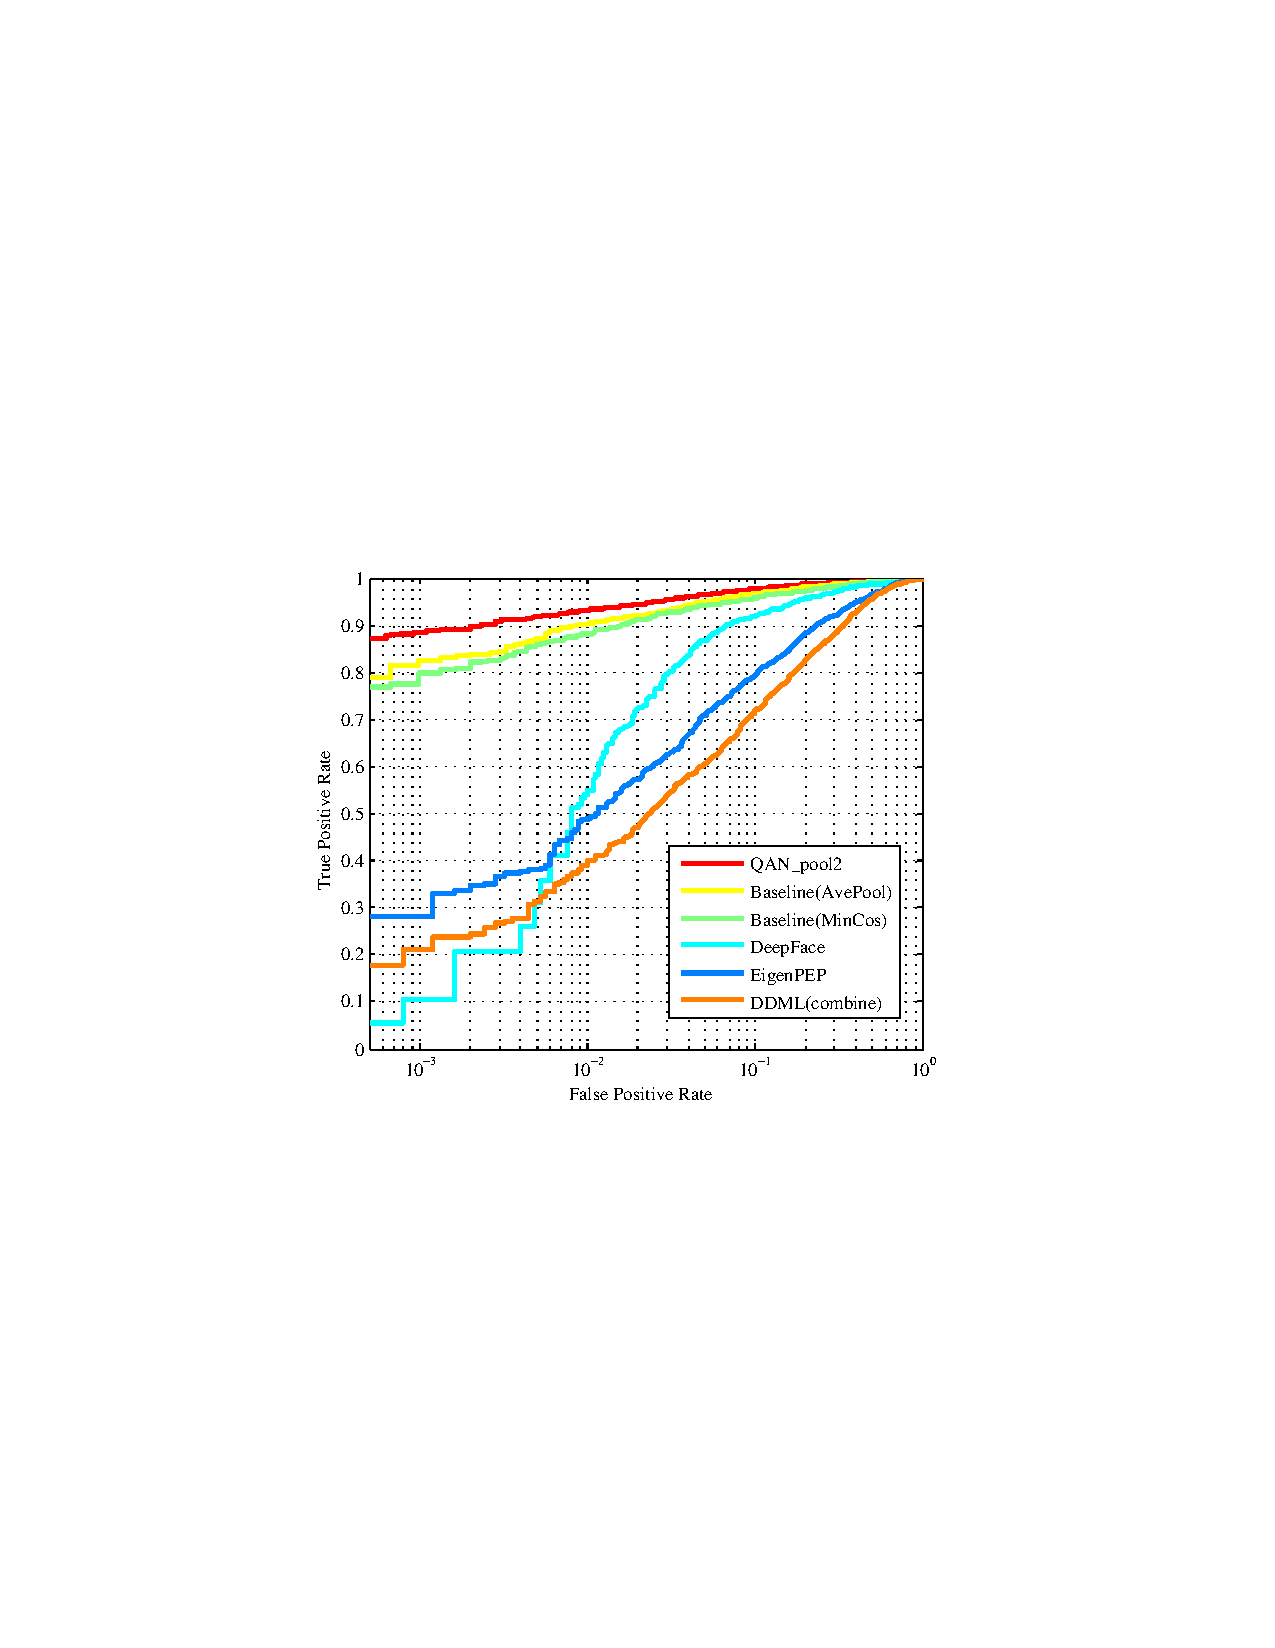
\includegraphics[height=4cm]{rocs.pdf}
  \caption{Average ROC curves of different methods on YouTube Face Dataset}
  \label{fig:rocs}
\endminipage\hfill
%\minipage{0.32\textwidth}
%\center
%  \includegraphics[width=5.5cm]{c5_experiment/cascade_num-tpr.pdf}
%  \caption{QAN's sensitivity to cascade number, analysed on YouTube Face Dataset.}
%  \label{fig:casnum2tpr}
%\endminipage\hfill
\minipage{0.35\textwidth}%
\center
  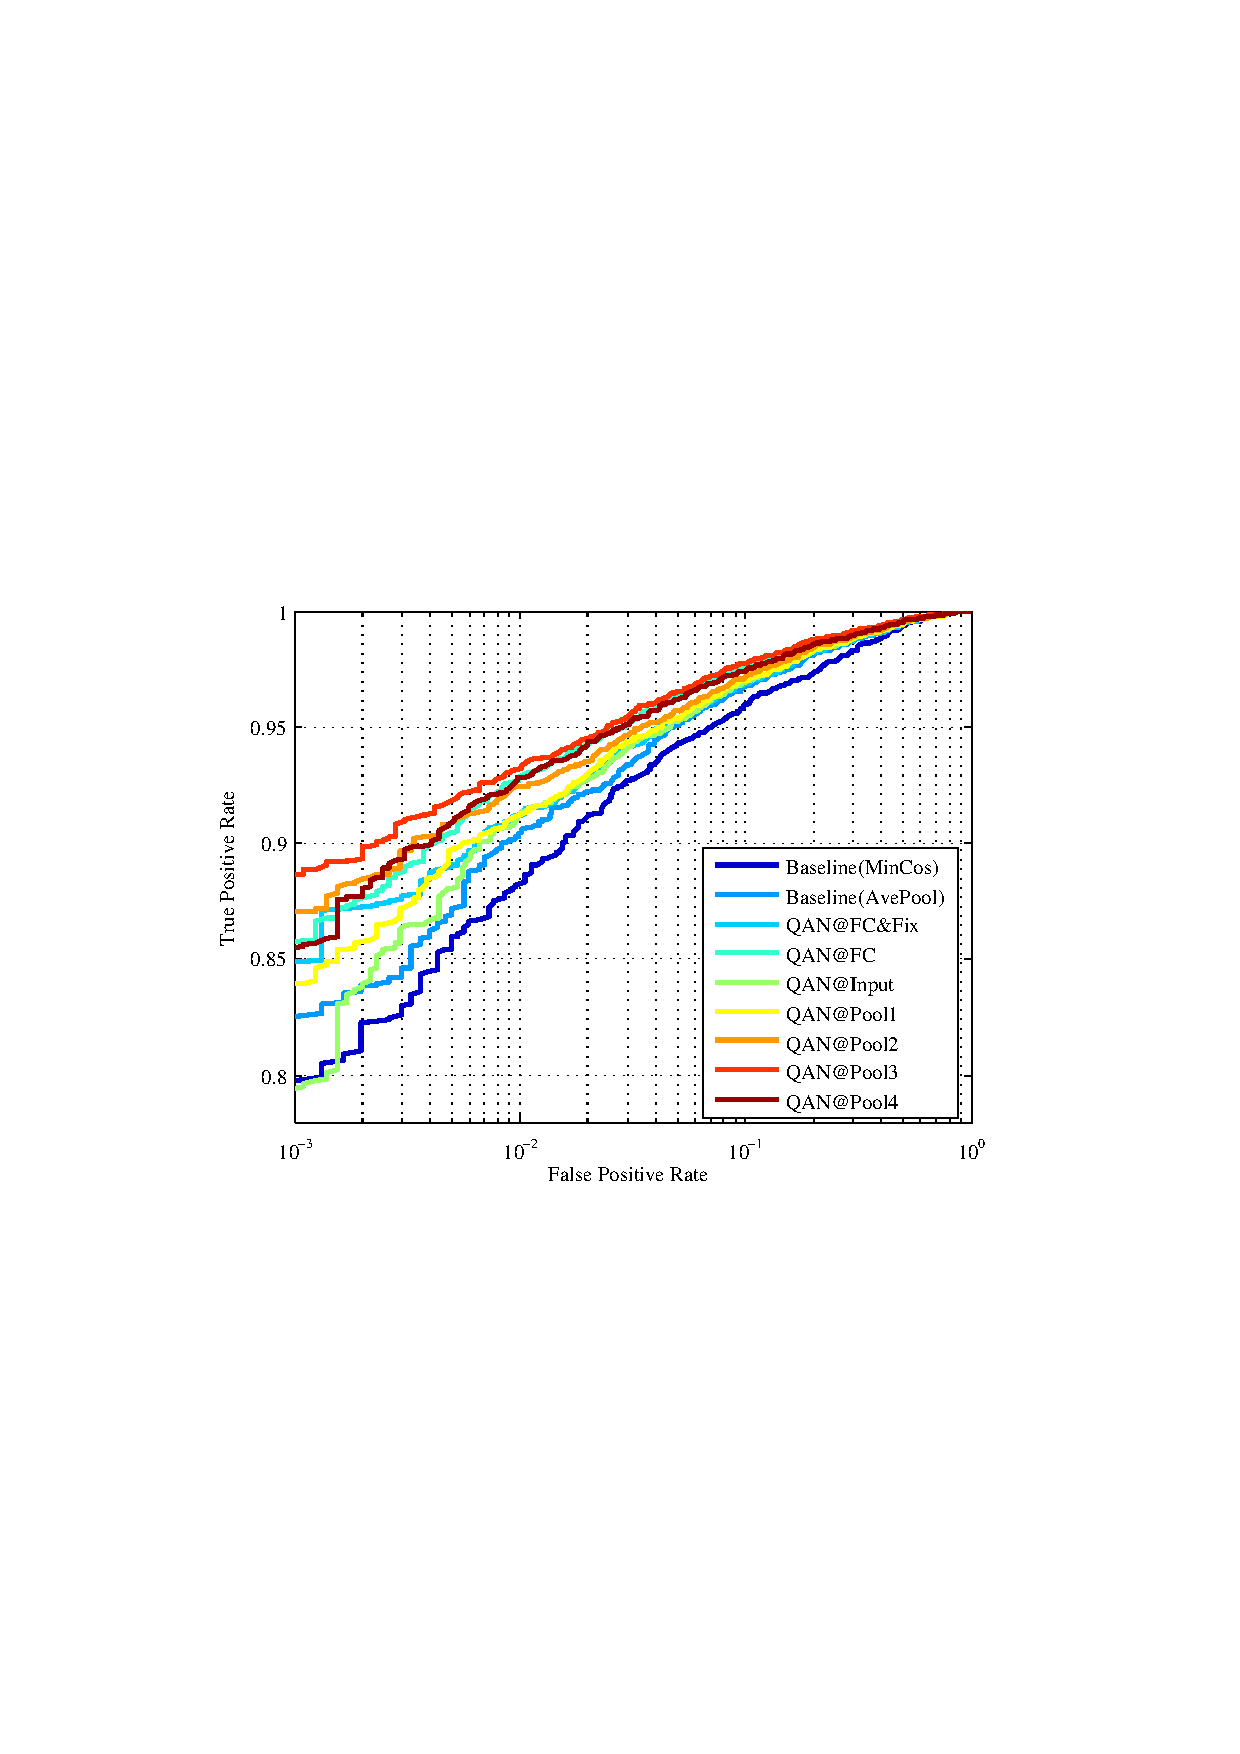
\includegraphics[height=4cm]{rocs_youtube_qanloc.pdf}
  \caption{ROC results for score generation part learned by different level of feature.}
  \label{fig:qanloc}
\endminipage
\minipage{0.32\textwidth}
\centering
  \includegraphics[height=4cm]{n4321-ok.pdf}
  \caption{QAN with human score performs better than the two baselines but worse than that scored by network.\label{fig:roc4321}}
\endminipage


\end{figure*}

\subsection{Unconstrained face verification}
\textbf{Datasets.} For face verification, we train our base model on extended version of VGG Face dataset~\cite{Parkhi15}, in which we extend the identity number from 2.6K to 90K and image number from 2.6M to 5M. The model is evaluated on YouTube Face Database~\cite{wolf2011face} and IARPA Janus Benchmark A (IJB-A) dataset. YouTube Face contains 3425 videos of 1595 identities. It is challenging in that most faces are blurred or has low resolution. IJB-A dataset contains 2042 videos of 500 people. Faces in IJB-A have large pose variance.

\textbf{Evaluation procedure.} We follow the 1:1 protocol in both two benchmarks and evaluate results using receiver operating characteristic (ROC) curves. Area under curve (AUC) and accuracy are two important indicators of the ROC. The datasets are evaluated using 10-fold cross-validation.

\textbf{Training details.}
All faces in training and testing sets are detected and aligned by a multi-task region proposal network as described in \cite{chen2016supervised}. Then we crop the face regions and resize them to $256\times 224$. After that, a convolutional neural networks with $256\times 224$ inputs are used for face verification. It begins with a 2-stride convolution layer, followed by 4 basic blocks, while each block has three 1-stride convolution layers and one 2-stride pooling layers. After that, a fully connected layer is used to get the final feature. Quality generation branch is built on top of the third pooling layer, where the spatial size of middle representation response is $256\times 16 \times 14$. We pre-train the network supervised by classification signal and then train the whole QAN.



\subsubsection{Results on YouTube Face and IJB-A benchmark}


\begin{table}[h]
\normalsize
  \centering
  \begin{tabular}{l|c|c}
    \hline
    Method & Accuracy(\%) &AUC \\
    \hline
       QAN   & \bf{96.17$\pm$ 0.09\%} & \bf{99.14$\pm$ 0.12\%} \\
       CNN+AvePool 	 & 95.46$\pm$ 0.07\% & 98.66$\pm$ 0.04\% \\
       CNN+Min(cos)  & 94.87$\pm$ 0.10\% & 98.37$\pm$ 0.06\% \\
    \hline
       NAN\cite{yang2016neural}			 & 95.52$\pm$0.06\% & 98.7\% \\
       FaceNet\cite{schroff2015facenet} 	& 95.12$\pm$0.39\% & - \\
       DeepID2+\cite{sun2015deeply}			& 93.2$\pm$0.2\% & - \\
       DeepFace-single\cite{taigman2014deepface}		& 91.4$\pm$1.1\% & 96.3\% \\
       EigenPEP\cite{li2014eigen}			& 84.8$\pm$1.4\% & 92.6\% \\
    \hline
  \end{tabular}

  \caption{Average accuracy and AUC of QAN on YouTube Face dataset, compared with baselines and other state-of-the-arts.}
  \label{tab:ytf}
\end{table}

\begin{table}[!htbp]
\footnotesize
  \centering
  \begin{tabular}{l|c|c|c}
    \hline
       TPR@FPR & 1e-3 & 1e-2  & 1e-1 \\
    \hline
       QAN 	& \bf{89.31$\pm$3.92\%} & \bf{94.20$\pm$1.53\%} & \bf{98.02$\pm$0.55\%} \\
       CNN+AvePool 		& 85.30$\pm$3.48\% & 93.81$\pm$1.44 & 97.85$\pm$0.61\% \\
       CNN+Min(cos) 	& 82.74$\pm$3.61\% & 92.06$\pm$1.98 & 97.29$\pm$0.67\% \\
    \hline
       NAN\cite{yang2016neural}		&78.5$\pm$2.8\% &89.7$\pm$1.0\% &95.9$\pm$0.5\% \\
       DCNN+metric\cite{chen2015end} 	& - & 78.7$\pm$4.3\% & 94.7$\pm$1.1\% \\
       LSFS\cite{wang2015face}				& 51.4$\pm$6.0\% & 73.3$\pm$3.4\% & 89.5$\pm$1.3\% \\
       OpenBR\cite{klontz2013open}				& 10.4$\pm$1.4\% & 23.6$\pm$0.9\% & 43.3$\pm$0.6\% \\
    \hline
  \end{tabular}
  \caption{TPRs of QAN at specific FPRs on IJB-A dataset, compared with baselines and other state-of-the-arts.}
  \label{tab:ijb}
%\end{scriptsize}
\end{table}

On YouTube Face dataset, it can be observed in Fig.~\ref{fig:rocs} and Table~\ref{tab:ytf} that the accuracy and AUC of our baselines are similar with the state-of-the-art methods such as FaceNet and NAN. Based on this baseline, QAN further reduces 15.6\% error ratio. Under ROC evaluation metric, QAN surpasses NAN by 8\% and DeepFace by 80\% at 0.001 FPR (false positive rate), which ensembles 25 models.

On IJB-A dataset, QAN significantly outperforms the state-of-the-art algorithm NAN by 10.81\% at 0.001 FPR, 4.5\% at 0.01 FPR and 2.12\% at FPR=0.1, as shown in Table~\ref{tab:ijb}. Compared with average pooling baseline, QAN reduces false negative rate at above three FPRs by 29.32\%, 6.45\% and 7.91\%.

Our experiments on the two tasks show that QAN is robust for set-to-set recognition. Especially on the point of low FPR, QAN can recall more matched samples with less errors.


%\subsubsection{QAN with different training data}

%We research into how number of identities, image number of each identity and frame number in each training batch influence the performance.

%As shown in Table~\ref{tab:insufdata}, in the first row block, we use all training data but different frame number in each training batch. For example, in the second line of this block begin with ``RS 4 images'',  we random select 4 images for each selected identity to training in each training batch. So the network's total batch size should be $3\times 4$, which are four images for `anchor', four images for `positive' and four images for ``negative''. Note that all images of a identity have the same probability to be trained. In the second block, we use same number in batch but different number of identities. only 500, 2k, 8k or 16k identities is selected to train our QAN. In the third block, we only use 4, 16, 32 or 128 training samples for each identity, which means identities who have more than 4, 16, 32 or 128 images are trained only part of their images.

%\begin{table*}[!htbp]
%\centering
%\begin{tabular}{|l|c|c|c|c|c|}
%\hline
%Strategy                                                                                         & Image Number & Identity Number & TPR@1E-3     & TPR@1E-2     & TPR@1E-1     \\ \hline
%Random Sample (RS) all images           & 90K          & 5M              & 88.67 & 93.18 & 97.42 \\
%RS 4 images                                                                           & 90K          & 5M              & 84.57        & 90.93        & 96.81        \\
%RS 16 images                                                                          & 90K          & 5M              & 87.13        & 92.65        & 97.22        \\
%RS 64 images                                                                          & 90K          & 5M              & 88.34        & 93.06        & 97.44        \\
%RS 128 images                                                                         & 90K          & 5M              & 88.59        & 93.24        & 97.4         \\ \hline
%RS 16 images, 0.5k identities   & 0.5k         & 137K            & 66.48        & 74.26        & 91.87        \\
%RS 16 images, 2k  identities        & 2k           & 588K            & 73.52        & 84.77        & 94.74        \\
%RS 16 images, 8k  identities                                                       & 8k           & 1.7M            & 78.81        & 88.38        & 95.26        \\
%RS 16 images, 16k identities                                                       & 16k          & 3M              & 83.79        & 90.92        & 96.45        \\ \hline
%Only Use (OU) 4 frames per identity   & 30K          & 120K            & 70.24        & 79.5         & 92.02        \\
%RS 16 images, OU 16 frames & 30K          & 480K            & 79.26        & 86.83        & 94.35        \\
%RS 16 images, OU 32 frames  & 30K          & 917K            & 84.95        & 90.45        & 96.22        \\
%RS 16 images, OU 128 frames & 30K          & 3.29M           & 87.09        & 92.49        & 97.18        \\ \hline
%\end{tabular}
%\caption{QAN's sensitivity to number of training data, analysed on YouTube Face Dataset.}
%\label{tab:insufdata}
%\end{table*}



\subsection{ Quality by QAN VS. quality by human}
\label{sec:humanscorebetter}
There is no explicit supervision signals for the cascade score generation unit in training. So another problem arises: is it better to use human-defined scores instead of letting the network learn itself? In YouTube Face experiment, we replace the quality score $Q(I)$ with volunteer-rated score and get the following result in Fig.~\ref{fig:roc4321}, which is better than the two baselines but inferior to the result of original QAN. It shows that $Q$ is similar with human thoughts, but more suitable for recognition. Quality score by human can also enhance the accuracy but is still worse than QAN's.



\subsection{Diagnosis experiments}
%Cascade number in quality generation part and 
Level of middle representation may affect the performance of QAN. We use YouTube Face to analyse this factor by comparing different configurations.

%\textbf{Cascade number.} We examine ROC performance with respect to the cascade number.  Fig.~\ref{fig:casnum2tpr} shows that the TPRs at FPR=1E-1 and FPR=1E-2 converge at 2-cascade while TPR at FPR=1E-3 converges at 3-cascade. This indicates that quality generation parts at higher levels can learn better weight metrics than that at low levels. Finally, the performance decreases at the 4-th cascade due to the over-fitting.


%\textbf{Feature level.} To discover which level of feature is better for weight learning in QAN, we compare 3-cascade QANs with different configurations. 
In the first configuration, the weight generation part is connected to the image. In the second to fifth configurations, weight generation part is set after four pooling layers in each block, respectively. In the sixth configuration, we connect weight generation part to a fully connected layer. For the final configuration, we fix all parameters before the final fully connection layer in the sixth configuration and only update parameters in weight generation part, which is taken as the seventh structure. To minimize the influence by parameters' number, the total size of different models is restricted to the same by changing the channel number. 

Results are shown in Fig.~\ref{fig:qanloc}. It can be found that the performance of QAN improves at the beginning and reaches the top accuracy at \texttt{Pool3}. The end-to-end training version of feature generation part with quality generation part performs better than that of fixed. So we can make the conclusion that 1) the middle level feature is better for QAN to learn and 2) significant improvement can be achieved by jointly training feature generation part and quality generation part.